% Chapter Template

\chapter{Implementing the PO-TITE-CRM trial design into ADePT-DDR} % Main chapter title

\label{Chapter2} % For referencing this chapter elsewhere, use \ref{Chapter2}

%----------------------------------------------------------------------------------------
%	SECTION 1
%----------------------------------------------------------------------------------------

\section{Introduction}

Worldwide there are approximately 600,000 new cases of Head and Neck Squamous Cell Carcinoma (HNSCC) each year \cite{stranskyMutationalLandscapeHead2011}. Of which, 12,000 occur in the UK with the most common forms of treatment being surgery, radiotherapy and/or chemotherapy \cite{cancerreaserchukHeadNeckCancers2017}. Radiotherapy is essential for the treatment of cancer, it has been estimated that more than 40\% of patients will receive radiotherapy at some point in their treatment \cite{roundRadiotherapyDemandActivity2013}. However, despite recent advancements in radiation techniques and the use of concomitant chemo radiotherapy, patients with solid tumours such as head and neck cancer have suboptimal cure rates \cite{cancerreaserchukHeadNeckCancers2017,cognettiHeadNeckCancer2008}. For those with advanced HNSCC primary radiotherapy with concurrent chemotherapy is often offered but, it has not been shown to improve survival in patients aged over 70 compared to radiotherapy alone \cite{pignonChemotherapyAddedLocoregional2000}. Therefore, any strategy to improve the efficacy of radiotherapy without increasing toxicity would have a significant impact on patient outcomes. 

DNA damage repair (DDR) inhibition is a potential technique which could be utilised as it potentiates the therapeutic effects of ionising radiation in cancer cells without a substantial increase in acute and late toxicity. Combining radiotherapy with DDR inhibition could improve clinical outcomes for these patients \cite{chalmersScienceFocusCombining2016}.  

The ADePT-DDR trial is a platform trial which aims to evaluate the safety and efficacy of different DDR agents, or different immunotherapy agents and/or DDR and immunotherapy combinations, together with radiotherapy in patients with HNSCC. The initial component of this trial is a single-arm dose-finding phase \RN{1}b/\RN{2}a trial investigating the Ataxia Telangiectasis and Rad3 Related (ATR) inhibitor AZD6738 in combination with radiotherapy. ATR inhibitors not only stop DNA repair but impairs the mechanism that allows for repairs to take place. Preclinical models have shown this double blocking to be effective in killing cancer cells \cite{meiAtaxiaTelangiectasiaRad3related2019}. 

Traditionally dose-finding trials aim to determine the maximum tolerated dose (MTD) of a treatment based on the cytotoxic assumption that the most toxic dose is the most efficacious. Rule-based or 'up and down' designs achieve this by escalating and de-escalating doses dependent on the observation of severe toxicity due to the drug,  commonly referred to as a dose-limiting toxicity (DLT). In the case of the 3+3 design escalation continues until at least two patients in a cohort of three or six experience a DLT. More explicitly, the MTD is the dose at which $\geq$33\% of patients experience a DLT \cite{letourneauDoseEscalationMethods2009}. Model-based designs such as the continual reassessment method (CRM) \cite{oquigleyContinualReassessmentMethod1990} work on a slightly different principle which assumes that the probability of toxicity monotonically increases with dose. One key difference with the CRM is that it iteratively changes dose, seeking some acceptable target probability of toxicity also referred to as the MTD. 

Due to the historical use of rule-based designs, the majority of the terminology used to describe them, and the ambiguity they raise, have been inherited by modern designs such as the CRM. The MTD in the context of a CRM is not the 'maximum' dose patients could tolerate but rather a dose in which there would be an acceptable target probability of a DLT occurring. For example, if the target is set at 25\% the MTD would be the dose at which there is a 25\% probability of experiencing a DLT. Rather than using the term MTD, the dose to be found will be referred to as the target dose (TD\%\%, where the \%'s are replaced by the target probability), i.e. TD25 would be the dose expected to be toxic in 25\% of patients.

The investigation of multiple-agent treatments, where the monotonicity assumption may not hold, is increasing in early phase trials. Finding the TD in combinations of treatments, compared to single-agents,  presents methodological challenges. Each drug individually may obey the monotonicity assumption, however, when combined, the ordering of doses in terms of toxicity may not be fully apparent. An order for a subset of the combined doses could be identified resulting in a partial order. Without a fully understood ordering it is uncertain which dose should be chosen in decisions of escalation and de-escalation and ultimately as the TD. This issue is not exclusively reserved for trials with multiple-agents. The monotonicity assumption may not hold for certain drugs in single-agent studies leading to partial orders of dose toxicity. This can occur in scenarios where multiple parameters of the treatment schedule are altered for each dose level. For example, either dose or treatment duration could be increased and even if patients receive an equal dose it would remain unclear as to if prolonged exposure to a lower dose is more toxic than short exposure to a higher dose, which implies a partial ordering of toxicity probabilities. 

Further methodological challenges revolve around the issue of late-onset toxicities. Typically, early phase trials implement a short window, post-treatment, to observe DLTs. This works well in situations where toxicities are likely to occur rapidly after treatment. However, this is not optimal for treatments that could cause late-onset toxicities such as radiotherapy. The aim here would be to incorporate a larger observation window to account for potential late-onset toxicities whilst also minimising the trial duration. 

Cheung and Chappel \cite{cheungSequentialDesignsPhase2000} introduced an extension to the CRM to deal with the issues of treatments that may cause late-onset toxicity. This design referred to as the time-to-event CRM (TITE-CRM), uses a weighted dose-response model to incorporate the time it takes for a DLT to occur in a patient. There have also been published trial designs to deal with the issues that arise from investigating combinations of treatments. Thall et al. \cite{thallDoseFindingTwoAgents2003} proposed an adaptive two-stage Bayesian design which utilises a parametric model of toxicity as a function of two doses. Yin and Yaun \cite{yinBayesianDoseFinding2009} present a Bayesian design that uses a copula regression model to evaluate the joint toxicity probabilities of combined drugs. The continual reassessment method for partial orders (PO-CRM) developed by Wages et al. \cite{wagesContinualReassessmentMethod2011} extends the CRM design by relaxing the assumption of monotonicity and by modelling different potential orders.  

Wages et al. \cite{wagesContinualReassessmentMethod2011, wagesUsingTimetoeventContinual2013} further developed their work on the PO-CRM to deal with late-onset toxicities by implementing a TITE component. This trial design, referred to as the time-to-event continual reassessment method in the presence of partial orders (PO-TITE-CRM) by the authors, was chosen to be used in ADePT-DDR. A search of PubMed, conducted on the 25th of July 2020, found six articles that had cited the PO-TITE-CRM design by Wages et al. \cite{wagesUsingTimetoeventContinual2013}. Five of these papers were methodological in nature, two of which only include the PO-TITE-CRM design in a brief introduction to current methodology before going on to present new Bayesian trial designs \cite{liuBAYESIANDATAAUGMENTATION2013, wheelerBayesianModelfreeApproach2019}. The other three papers were authored by Wages. The first of which details practical considerations and specifications for the PO-CRM design, the TITE variant is only cited as the source of an example which is being used \cite{wagesSpecificationsContinualReassessment2013}. One paper presents an R package 'pocrm' \cite{wagesPocrmRpackagePhase2013, wagesPocrmDoseFinding2019}, the package is only capable of analysing the PO-CRM design, similarly, the TITE variant is only referenced as it illustrates the issue of partial ordering. The last methodological paper by Wages et al. \cite{wagesPracticalDesignsPhase2016} presents three different methods for phase \RN{1} studies of drug combinations one of which is the PO-CRM however, PO-TITE-CRM is only mentioned as an extension to this design. A key message in this paper is the fact that novel methodologies are constantly emerging but are rarely implemented in practice. The last paper is a protocol paper that is investigating a combination of treatments however, it is only escalating dose in one of the drugs \cite{lesueurPhaseIIaStudy2019}. The PO-TITE-CRM paper is cited but it appears as if another variant of the TITE-CRM is being used. This is just a brief review of the current literature but it seems that the PO-TITE-CRM has rarely been used or discussed since its inception. 

Section \ref{section2.2} will detail how the PO-TITE-CRM works. Section \ref{section2.3} discusses the justification for implementing the design into the ADePT-DDR trial and our experiences doing so.  

%----------------------------------------------------------------------------------------
%	SECTION 2
%----------------------------------------------------------------------------------------
\section{The PO-TITE-CRM Design}
\label{section2.2} %first number is the chapter number, second number is section number, third is subsection etc...

Wages et al. \cite{wagesUsingTimetoeventContinual2013} introduced the PO-TITE-CRM design which builds directly upon the PO-CRM design by incorporating a TITE component into the dose toxicity model. The aim of which is to determine the target dose for combinations of drugs where the monotonicity assumption does not hold, in a setting where late-onset toxicities are possible.

To help understand partial ordering consider an example of an early phase trial investigating the combination of two agents. Drug A which consists of three doses (0.25, 1.0, 1.5 mg/day) and drug B which consists of two doses (1.0, 1.5 mg/day), for a total of six drug combinations $d_{1}$, ..., $d_{6}$ (Table \ref{tab_adept:ex_drug_combo}). For each drug independently we assume they have a monotonic dose-toxicity curve however, the ordering of toxicity probabilities for some of the treatment combinations is unknown. Specifically, we can say $d_{1}$ is less toxic than $d_{2}$ even the dose of drug B is the same as the dose of drug A increased. The same can be said for $d_{2}$ and $d_{3}$. The order between $d_{4}$, $d_{5}$ and $d_{3}$ is not known because the dose of drug A decreases whilst the dose of drug B increases. Assessing all these potential order toxicity relationships leaves 5 possible orderings. 

\begin{enumerate}
	\centering
	\item $d_{1} \rightarrow d_{2} \rightarrow d_{3} \rightarrow d_{4} \rightarrow d_{5} \rightarrow d_{6}$
	\item $d_{1} \rightarrow d_{2} \rightarrow d_{4} \rightarrow d_{3} \rightarrow d_{5} \rightarrow d_{6}$
	\item $d_{1} \rightarrow d_{2} \rightarrow d_{4} \rightarrow d_{5} \rightarrow d_{3} \rightarrow d_{6}$
	\item $d_{1} \rightarrow d_{4} \rightarrow d_{2} \rightarrow d_{3} \rightarrow d_{5} \rightarrow d_{6}$
	\item $d_{1} \rightarrow d_{4} \rightarrow d_{2} \rightarrow d_{5} \rightarrow d_{3} \rightarrow d_{6}$
\end{enumerate}

\begin{table}[h!]
	\centering
	\caption{Example of drug combinations for a trial investigating two agents.}
	\label{tab_adept:ex_drug_combo}
	\begin{tabular}{lcccccc}
		\hline  & \multicolumn{6}{c}{\textbf{Drug combinations}}  \\
		\textbf{Agent} & $d_{1}$ & $d_{2}$ & $d_{3}$ & $d_{4}$ & $d_{5}$ & $d_{6}$ \\ \hline
		A (mg/day) & 0.25 & 0.5 & 1.0 & 0.25 & 0.5 & 1.0         \\
		B (mg/day) & 1.0  & 1.0 & 1.0 & 1.5  & 1.5 & 1.5         \\ \hline
	\end{tabular}
\end{table}

Using the notation of Wages et al. \cite{wagesContinualReassessmentMethod2011,wagesUsingTimetoeventContinual2013}, let $M$ denote the number of possible orders and $Y$ be an indicator of a toxicity event. Then for a trial investigating $k$ combinations, $d_{1}$,...,$d_{k}$, the dose for the $j$th patient, $X_{j}$, $j$ = 1,...,$n$ can be thought of as random $x_{j} \in (d_{1}, ..., d_{k})$. For a specific ordering $m$, $m = 1,...,M$ the toxicity probability $R(x_{j})$ is modelled by 
\begin{equation}
R(x_{j}) = P(Y_{j} = 1 | X_j = x_j) = E(Y_j|x_j) \doteq \phi_m(d_i,w,a) = w\psi_m(d_i,a)
\end{equation}
for  a weighted dose response model $\phi_m(d_i,w,a)$ and $a \in A$, where $A = (-\infty, \infty)$. The weight, $w$ as defined by Cheung and Chappel \cite{cheungSequentialDesignsPhase2000}, is a function of the time-to-event of each patient and is incorporated linearly with the dose toxicity model $\psi$ so that $0 \leq w \leq 1$. Each patient is followed for a fixed amount of time $T$. Let $U_j$ represent the time-to-toxicity of patient $j$. Then for $u \leq T$, 
\begin{equation}
	P(U_j \leq u ) = P(U_j \leq u |U_j \leq T)P(U_j \leq T) \equiv w(u;T) \psi_m(d_i,a).
\end{equation}
For simplicity we will refer to the weight function $w(u;T)$ as $w$. The weight function will have to be decided upon by the trials team, dependent on the scenario, a simple linear function or a more complex adaptive weights function could be utilised. There are also several working dose models which could be used for $\psi$, Wages et al. \cite{wagesUsingTimetoeventContinual2013} present their design with the power parameter model given by 
\begin{equation}
	\psi_m(d_i,a) = \alpha_{mi}^{exp(a)} i = 1,...,k; m = 1,...,M.
\end{equation}
Here $0 < \alpha_{m1} < ... < \alpha_{mk} < 1$ are the prior estimates of toxicity probabilities, or skeleton, for each potential ordering. Furthermore, prior probabilities are assigned to each order $M$ to account for any prior information regarding the plausibility of each model such that, $p(m) = \{p(1),...,p(M)\}$, where $p(m) \geq 0$ and $\sum_mp(m)=1$. When all orders are equally likely or there is no prior information available on possible orderings the prior is discretely uniform and would be $p(m) = 1/M$. 

A Bayesian framework is used and a prior probability distribution $g(a)$ is assigned to the parameter $a$. The ordering with the largest prior probability is selected as the starting ordering, in the scenario where all priors are equal an ordering is selected at random, subsequently a starting dose is also chosen. After $j$ patients have been entered into the trial data is collected in the form of $\Omega_j = \{x_1,y_1, ..., x_j,y_j\}$. A weighted likelihood for the parameter $a$ is used to establish running probabilities of toxicity for each treatment combination. The weighted likelihood under ordering $m$, is given by 
\begin{equation}
\tilde{L}_m(a|\Omega_j)=\prod_{l=1}^{j}\phi_m^{y_l}(d_l,w_l,a)\{1-\phi_m(d_l,w_l,a)\}^{(1-y_l)}
\end{equation} 
which can be used to generate a summary value $\hat{a}_{mj}$, for $a$, for each ordering. With the likelihood and the data $\Omega_j$, the posterior density for $a$ can be calculated using 
\begin{equation}
	\tilde{f}_m(a|\Omega_j)=\frac{\tilde{L}_m(a|\Omega_j)g(a)}{\int_{A}\tilde{L}_m(a|\Omega_j)g(a)da}
\end{equation}
This can then be used to establish posterior probabilities of the orderings given the data as 
\begin{equation}
\tilde{\pi}(m|\Omega_j)=\frac{p(m)\int_{A}\tilde{L}_m(a|\Omega_j)g(a)da}{\sum_{m=1}^{M}p(m)\int_{A}\tilde{L}_m(a|\Omega_j)g(a)da}.
\end{equation}
We select the single ordering, $h$, with the largest posterior probability along with its associated working model $\psi_h(d_i,a)$ and generate toxicity probabilities for each dose level. Once the $j$th patient has been included the posterior probability of DLT can be calculated for $d_{i}$ so that
\begin{equation}
	\hat{R}(d_i) = \psi_h(d_i,\hat{a}_{hj}); \; \hat{a}_h = \int_{A}a\tilde{f}_h(a|\Omega_j)da.
\end{equation}

In turn, the dose level $x_j \in \{d_1,...,d_k\}$ assigned to the ($j+$1)th patient is the dose, $d_i$, which minimises 
\begin{equation}
\label{eq_adept:crm_min}
	\triangle(\hat{R}(d_i),\theta) = |\hat{R}(d_i)-\theta|, \; i=1,...,k
\end{equation}
where $\theta$ is the target toxicity rate. Similarly, once all patients have been recruited and observed and the trial ends, the target dose (TD$\theta$) is the dose, $d_{i}$, which minimises (\ref{eq_adept:crm_min}).

%----------------------------------------------------------------------------------------
%	SECTION 3
%-------------------------.

\section{PO-TITE-CRM in ADePT-DDR}  
\label{section2.3}%first number is the chapter number, second number is section number, third is subsection etc..
The decision to implement PO-TITE-CRM into ADePT-DDR was made by Piers Gaunt (PG) after discussions with other statisticians Kristian Brock (KB) and Daniel Slade (DS), as well as the chief investigator and other co-investigators. The design was chosen as the toxicity probabilities of the dose levels weren't monotonically increasing which restricts the use of most early phase designs such as the CRM. Additionally, the design also handles late-onset toxicities which would be an issue in ADePT-DDR due to the treatment involving radiotherapy. The availability of software to conduct the trial was also a factor that was considered. The R package 'pocrm' \cite{wagesPocrmRpackagePhase2013} only provides a means for implementing the PO-CRM design but the easy accessibility to this code meant that it could be extended to include the TITE component.  

The intended use of this design is for dose-finding in combinations of therapies, as this is the source of the partial ordering issue. ADePT-DDR however, is a unique implementation of the design as even though it involves a combination of therapies (radiotherapy and AZD6783) the dose of radiotherapy is fixed and dose-finding is only planned for AZD6783. PO-TITE-CRM is still applicable in this case as the dose levels for AZD6783 are partially ordered. 

A two-stage PO-TITE-CRM will be used to find the TD25 of AZD6783. This will be determined by dose-limiting toxicities evaluated by Common Terminology Criteria for Adverse Events (CTCAE) v5.0 and Radiation Therapy Oncology Group (RTOG) late toxicity score. The binary DLT events are pre-defined by a variety of grade 3-4 adverse events notably, haematological, cardiovascular and gastrointestinal/hepatic toxicities as well as significant non-haematological events and specific treatment-related toxicities. DLTs will be monitored for the duration of treatment (seven weeks) and up to a year post-treatment. 


A maximum of 60 patients will be recruited for the dose-finding aspect of this trial and up to 20 patients as controls. Controls will be utilised to make comparisons for secondary outcomes such as survival and efficacy. Cohorts of three patients will be recruited and assigned to dose levels chosen by the PO-TITE-CRM. Controls will be recruited in the interim period between the recruitment of the third patient in a cohort and the completion of the minimum follow-up period.    

%-----------------------------------
%	SUBSECTION 3.1
%-----------------------------------
\subsection{Partial Ordering in Practice}
\label{section2.3.1}%first number is the chapter number, second number is section number, third is subsection etc..

Each patient entered into ADePT-DDR will receive fixed dose radiation, totalling 70 Gy in 35 fractions over seven weeks. For the dose-finding aspect we investigate six doses of AZD6783 detailed in table \ref{tab_adept:AZD_dose_levels}. Treatment dose and duration to be selected for dose level 3 will be determined based on a combination of data observed, adverse events and compliance. The issue of partial ordering stems from dose levels 2a and 2b, which can be seen in Figure \ref{fig_adept:AZD_dose_levels}. The increased duration of 2a and increased dose of 2b mean they are both more toxic than dose level 1. However, when comparing 2a and 2b it is unknown whether the increase in duration or dose will be more toxic. Hence there are two possible orderings for ADePT-DDR. 

\begin{enumerate}
	\centering
	\item $d_{-1} \rightarrow d_{0} \rightarrow d_{1} \rightarrow d_{2a} \rightarrow d_{2b} \rightarrow d_{3}$
	\item $d_{-1} \rightarrow d_{0} \rightarrow d_{1} \rightarrow d_{2b} \rightarrow d_{2a} \rightarrow d_{3}$
\end{enumerate}

\begin{table}[h!]
    \centering
	\caption{ADePT-DDR dose levels and duration of treatment for AZD6783.}
	\label{tab_adept:AZD_dose_levels}
		\begin{tabular}{ccccc}
			\hline 
			\multicolumn{1}{p{1.5cm}}{\centering \textbf{Dose} \\ \textbf{Level}} & \multicolumn{1}{p{3cm}}{\centering \textbf{AZD6783 Daily} \\ \textbf{dose (mg BD)}} &
		    \multicolumn{1}{p{1.5cm}}{\centering \textbf{Weeks} \\ } &
			\multicolumn{1}{p{1.5cm}}{\centering \textbf{Duration} \\ \textbf{(days)}} &
			\multicolumn{1}{p{3.5cm}}{\centering \textbf{Radiotherapy} \\ } 
			\\\hline
			-1 & 20 & 1 & 5 & 70 Gy/ 35 F \\
			 0 & 20 & 1\&4 & 10 & 70 Gy/ 35 F \\
			 1 & 40 & 1\&4 & 10 & 70 Gy/ 35 F \\
			2a & 40 & 1,2,4\&5 & 20 & 70 Gy/ 35 F \\
			2b & 80 & 1\&4 & 10 & 70 Gy/ 35 F \\
			\multirow{2}{*}{3} & 120 & 1\&4 & 10 & 70 Gy/ 35 F \\
			& 80 & 1,2,4\&5 & 20 & 70 Gy/ 35 F \\ \hline
		\end{tabular}
\end{table}

\begin{figure}[h!]
	\caption{ADePT-DDR dose levels across dose and duration.}
	\label{fig_adept:AZD_dose_levels}
	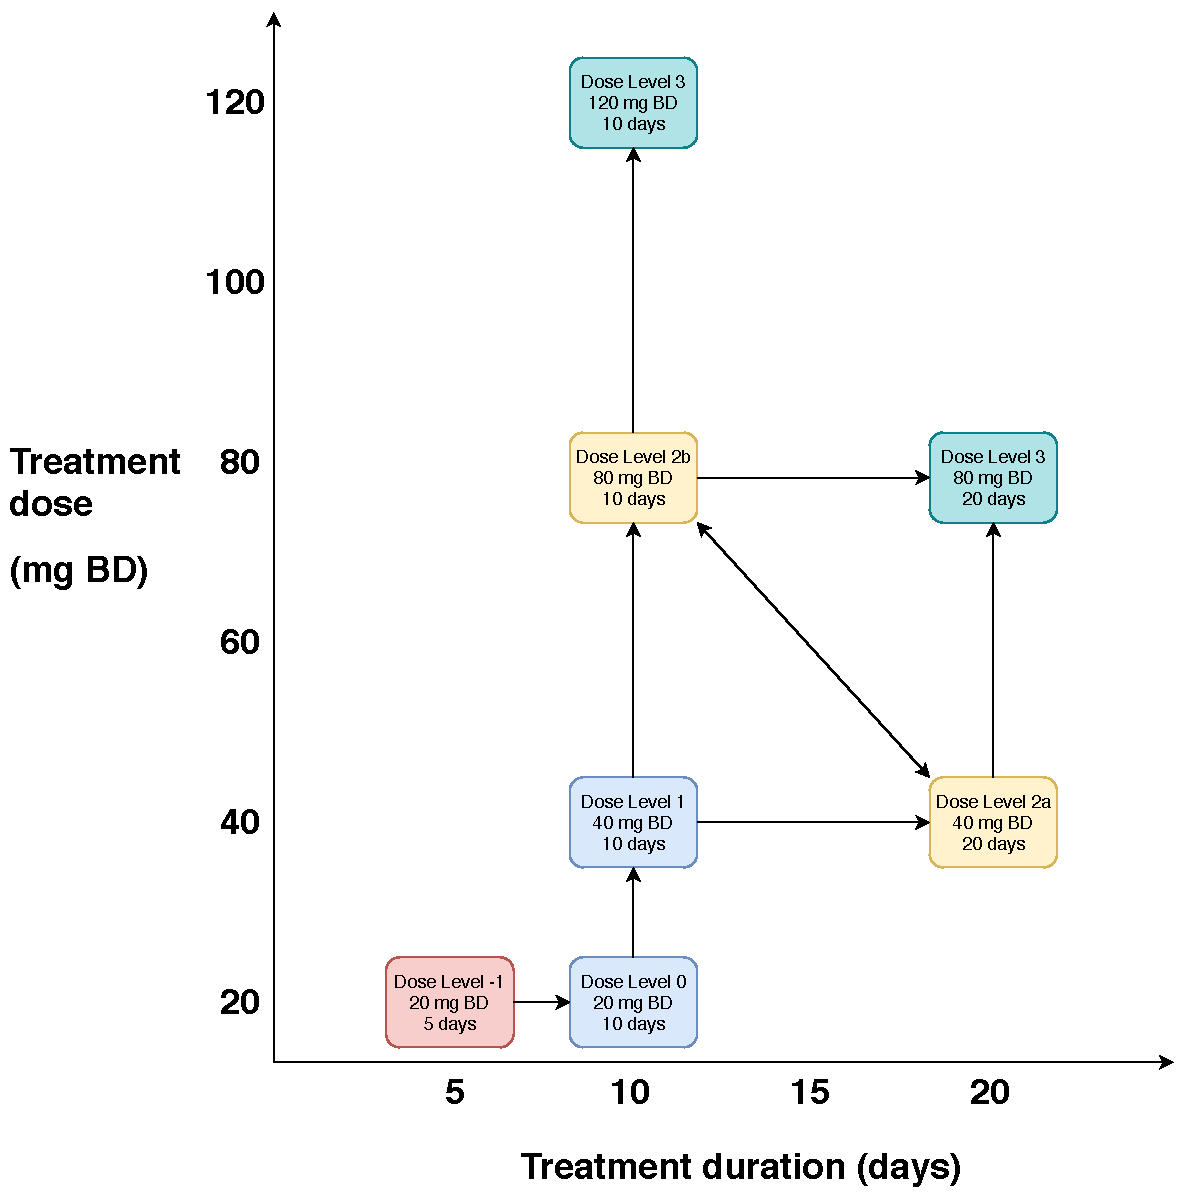
\includegraphics[width=\textwidth]{AdeptDoseCombos}
\end{figure}

Preliminary designs of the trial included only five dose levels and planned to use dose level 0 as the starting dose. During the trial design phase it was decided a new lower dose (dose level -1) would be introduced to allow for de-escalation if the initial dose was found to be too toxic. Dose escalation/de-escalation for subsequent cohorts would be determined from the two-stage PO-TITE-CRM. A two-stage design allows for escalation according to a pre-defined escalation scheme similar to a '3+3' design. The first stage dictates that if no DLT's are observed in the current cohort the dose allocated to the next cohort is the following dose in the escalation scheme. Dose levels continue to be incremented in this fashion until the first DLT is observed. In stage two, dose levels are determined by the PO-TITE-CRM.

Typically CRM designs begin by testing the first patient, or cohort, at the prior guess of TD. However, clinicians may have safety concerns beginning the trial at higher dose levels as well as escalating to higher dose levels without testing lower ones. Investigators in ADePT-DDR expressed similar concerns as such a two-stage design was adopted. The escalation scheme used in stage one of ADePT-DDR will follow that of the first ordering ($d_{-1} \rightarrow d_{0} \rightarrow d_{1} \rightarrow d_{2a} \rightarrow d_{2b} \rightarrow d_{3}$). If patients in the first cohort (assigned to dose level 0) don't experience a DLT the next cohort will be allocated to dose level 1 and then if no DLTs are observed again the third cohort will be allocated to dose level 2a and so on and so forth. The dose escalation scheme was determined based on the prior probabilities of toxicity generated for each dose level.  

Information elicited from the investigators helped generate prior probabilities of toxicity for each dose level. They believed that dose level 2b would be the TD25 with 2a being less toxic. This was used in conjunction with the getprior function from the dfcrm R package \cite{cheungDfcrmDoseFindingContinual2019} which yielded priors of 0.012, 0.036, 0.084, 0.157, 0.25 and 0.355 for dose levels -1, 0, 1, 2a, 2b and 3 respectively. Prior probabilities are also required for the plausibility of each model and even though the clinicians think that 2b will be more toxic than 2a there is no clear evidence and still a lot of uncertainty. As such it is sensible to assume a plausibility probability of 0.5 for each ordering, implying both orders are equally likely to be the true ordering of these dose levels. 

%-----------------------------------
%	SUBSECTION 3.2
%-----------------------------------
\subsection{The TITE component}
\label{section2.3.2}%first number is the chapter number, second number is section number, third is subsection etc..

The observation window for this trial will be longer as the combination of radiotherapy with AZD6738 is anticipated to cause late-onset toxicity. The Acute DLT observation period is 84 days (12 weeks) post radiotherapy end with a minimum of 56 days (8 weeks) for the last patient of each cohort. However, patients will continuously be monitored for occurrence of DLT for at least 84 days (12 weeks), i.e. at least 84 days (12 weeks) from the end of radiotherapy. Th full window will last for 365 days (52 weeks).

The TITE component incorporates a weighting contribution for each patient dependent on how long that patient has been evaluable in the study. This allows a patient to be evaluated once they have been observed for the minimum DLT period of 56 days (8 weeks). The weighting at this point is 60\% rising to 80\% at 84 days (12 weeks). A patient will not contribute fully to the model until they have completed 365 days (52 weeks) follow up (or have experienced a DLT at any stage in which case they will be weighted as a whole contribution). Linear weighting functions will be employed for any patient with a length of follow up between these three time points. One weighting function to calculate weight from 56-84 days (8-12 weeks) and another for weights from 84-365 days (12-52 weeks). For the weighting function $w(u;T)$ where $u$ is the time-to-toxicity of patient $j$ and $T$ is the time period, let $t_1, t_2, t_3$ take values 56, 84 and 365 respectively such that $T \in (t_1, t_2, t_3)$. Then for $t_1 \leq u \leq t_3$
\begin{equation}
w(u;T) = 0.6 + 0.2\frac{min(u-t_1,t_2 - t_1)}{t_2 - t_1} + 0.2\frac{max(0, u - t_2)}{t_3-t_2}.
\end{equation} 
All patients will have a minimum weight of 60\% as that is the prescribed weighting to the  minimum follow up period before dose escalation/de-escalation decisions can be made. For each additional week the patient is observed, without a DLT occurring, between weeks 8 and 12 their weighting increases by 5\%. Similarly for each week between 12 and 52 weeks, without a DLT, weighting increases by 0.5\%.

The TITE-CRM originally presented by Cheung and Chappel \cite{cheungSequentialDesignsPhase2000} did not incorporate a minimum follow-up period and their design allowed for the continual recruitment of patients whenever they became available. There are some practical considerations which make this infeasible. The model would need to be run each time a new patient entered the study which requires statistical input hence the introduction of cohorts. Clinicians may also have safety concerns if we see rapid recruitment at the start of the trial and the model keeps escalating so we impose a minimum follow-up period. Initially this was set at 12 weeks (at 80\% weighting) however, statisticians AP and PG  pointed out that dose escalation/de-escalation decisions would have to take place 19 weeks (7 weeks treatment and 12 weeks follow-up) after recruitment of the third patient in the cohort. Dependent on the recruitment rates this could extend the duration of the trial and negates the benefits of using a TITE design. The investigators aslo agreed this was too long and settled on lowering this period to 8 weeks (at 60\% weighting) whilst also including the original 12 week weighting of 80\%.

%Additional rules were implemented into the design for safety and early stopping.  
%Additional 
%
%Further considerations were made

%-----------------------------------
%	SUBSECTION 3.3
%-----------------------------------
\subsection{Stopping Rules}
\label{section2.3.3}%first number is the chapter number, second number is section number, third is subsection etc..

A practical modification was included to allow for early stopping of the trial if there is sufficient evidence that the TD has been reached. Sufficient evidence is achieved once 15 patients (five cohorts) have been treated at the same dose level and the model allocates that dose level again to a sixth cohort. This rule evolved from the original designs of the trial which involved 30 patients with a dose expansion cohort to ensure at least 15 patients were treated at the TD. 

Initial simulations highlighted the inadequacy of these design parameters as operating characteristics for various scenarios were poor, specifically in terms of correct TD selection. Clinicians explained the inclusion of the dose expansion cohort was to ensure the dose-finding aspect of the trial did not take a large amount of time whilst also allowing safety to be assessed at the TD. In order to ensure that a reasonable amount of patients would be treated at the TD, the trial wouldn't take longer than necessary and operating characteristics improved, the sample size was increase and this rule was introduced.

A rule was also implemented to allow for early termination of the trial in the case of excess toxicity at the lowest dose. If the posterior probability of DLT at the lowest dose is higher than 0.35 with a probability of 80\% and has been tested the trials safety committee will be alerted and will recommend if the trial should be stopped. As the trial starts at dose level 0, which is not the lowest dose, it is possible for the trial to recommend terminating without ever allocating patients to the lowest dose level. As such it was decided early termination would only occur once at least 3 patients (1 cohort) have been allocated dose level -1. 

%-----------------------------------
%	SUBSECTION 3.
%-----------------------------------
\subsection{Operating Characteristics}
\label{section2.3.4}%first number is the chapter number, second number is section number, third is subsection etc.. 

Simulations were continually utilised during the design process of the trial to assess how various changes impact the overall performance. These changes to design features such as the sample size, weight function and stopping rules helped inform decisions which led to the final design.  

Functions from pocrm package in R \cite{wagesPocrmRpackagePhase2013, wagesPocrmDoseFinding2019} were modified in order to perform simulations and conduct the trial. The majority of work involved integrating the TITE component and the stopping rules into the code. In standard CRM designs a binary outcome for toxicity is generated for each patient based on a pre-specified true DLT rates for the dose they are assigned. Adding the TITE component means the time the toxicity occurs also has to be generated, the simulation must also track this time and incorporate this information into the PO-TITE-CRM model when it needs to make dose allocation decisions for the next cohort. We defined multiple scenarios to reflect various real life possibilities in order to assess the designs performance.  

Standard scenarios to run involve adjusting the true DLT rates to reflect each dose being the TD25. For each of these we calculate the probability of selecting each dose as the TD25. It would be expected the dose with the highest probability of being selected has its true DLT rate set at 25\% to match the target rate. A high probability of selection for the correct dose implies the design works well in the specified scenario. Additional characteristics such as the average number of patients at each dose level are also investigated. This can be used to look at how many patients may potentially be allocated to a toxic dose. It is also necessary to consider performance when all doses are too toxic, here we would want the design to recommend stopping early. Usually the true DLT rates used to define these scenarios abide by the monotonicity assumption. Due to the partial ordering we consider scenarios in which the true DLT rates follow both orders. For trials with a large amount of orders it may be unfeasible to run so many simulations. However, as ADePT-DDR only has two orders we explored all scenarios for each ordering.

We simulated 2000 trials for each scenario using the finalised design detailed in section \ref{section2.3}. A fixed recruitment rate of one patient per month was utilised. The occurrence of DLT's were randomly generated for patients in each cohort using a Bernoulli distribution with the probability set at the true DLT rate for the cohorts assigned dose level in the specific scenario. For patients who had a DLT occur, the time at which the DLT occurred was randomly generated using a uniform distribution which spanned the start of treatment to the end of follow-up.  

Table \ref{tab_adept:OCorder1} details simulations for eight scenarios to test the performance of the PO-TITE-CRM design using true DLT rates which reflect the first ordering. We analyse scenarios where each dose is the TD25 (scenarios 1-6) and when all doses are too toxic (scenario 8). Additionally, we also investigate performance under conditions where the probability of DLT is fairly similar between doses (scenario 7). This is a notoriously difficult circumstance for CRM designs to deal with as the limited number of patients and events at each dose make it hard to accurately estimate toxicity probabilities if they are similar. Simulation results for ordering 2 are shown in Table \ref{tab_adept:OCorder2} where dose level 2a is considered more toxic than 2a. This is achieved by altering the true DLT rates so 2b has a lower probability of DLT compared to 2a. 

Ideally we want the probability of selection for the dose allocated at TD25 to be as high as possible and greater than other dose levels. For scenarios 1-7 the TD25 is highlighted in bold along with results from the simulations. However, for scenario 8 where all doses are too toxic we expect the trial to terminate early, here 'stop' should be selected and its associated probability of stopping is shown in bold. 

In scenarios 1 - 6 (Table \ref{tab_adept:OCorder1}), this design correctly selects the TD25 with probabilities between 44\% and 79\%, under the assumption 2b is more toxic than 2a. Likewise, for the ordering where 2a is more toxic than 2b, scenarios 9-14 (Table \ref{tab_adept:OCorder2}) have probabilities between 43\% and 78\% of correctly selecting the TD25. Correct selection probabilities are generally higher when the TD25 is at the first and last dose levels compared to dose levels 2a and 2b. However, these dose levels are still chosen with the highest probability as the TD25 in their given scenarios. For scenarios 7 and 15, the probabilities of toxicity are equally spaced, approximately 5\% apart. This is a relatively diffcult scenario for dose-finding studies to handle. The probability of selecting the TD25 is 26\% and 30\% for orderings 1 and 2 respectively. In scenarios 8 and 16, where all the doses are too toxic, the design very seldom allocates patients higher than the first three doses and there is a high chance (73\%) that the trial will recommend early stopping.



\begin{table}[h!] % OC for order 1 
	
	\caption[Operating Characteristics for ordering 1]{\label{tab_adept:OCorder1} Operating Characteristics of the two-stage PO-TITE-CRM (with true DLT rates that imply 2b is more toxic than 2a) based on 2000 simulated trials. Definitions: DLT: Dose-limiting toxicity. P(select):
	Probability of selecting a dose as the TD25.}
	\centering
	\begin{singlespace}
	\resizebox{\linewidth}{!}{
		\begin{tabular}[t]{ccccccccc}
			\toprule
			\multicolumn{2}{c}{ } & \multicolumn{6}{c}{Dose Levels} \\
			\cmidrule(l{3pt}r{3pt}){3-8}
			&  & -1 & 0 & 1 & 2a & 2b & 3 & Stop\\
			\midrule
			Scenario & Prior DLT & 0.01 & 0.04 & 0.08 & 0.16 & 0.25 & 0.35 & \\
			\cmidrule{1-9}
			\rowcolor{gray!6}   & True DLT rate & \textbf{0.25} & 0.4 & 0.45 & 0.5 & 0.55 & 0.6 & \\
			
			\rowcolor{gray!6}   & P(select) & \textbf{0.67} & 0.18 & 0.05 & 0 & 0 & 0 & 0.10\\
			
			\rowcolor{gray!6}   & \% of patients & \textbf{39} & 32 & 21 & 6 & 3 & 0 & \\
			
			\rowcolor{gray!6}  \multirow{-4}{*}{\centering\arraybackslash 1: TD25 @-1} & Mean number of patients & \textbf{10.03} & 8.26 & 5.34 & 1.65 & 0.68 & 0.06 & \\
			\cmidrule{1-9}
			& True DLT rate & 0.12 & \textbf{0.25} & 0.4 & 0.45 & 0.5 & 0.55 & \\
			
			& P(select) & 0.23 & \textbf{0.51} & 0.2 & 0.03 & 0.02 & 0 & 0.01\\
			
			& \% of patients & 17 & \textbf{35} & 29 & 11 & 6 & 1 & \\
			
			\multirow{-4}{*}{\centering\arraybackslash 2: TD25 @0} & Mean number of patients & 5.19 & \textbf{10.49} & 8.74 & 3.31 & 1.77 & 0.28 & \\
			\cmidrule{1-9}
			\rowcolor{gray!6}   & True DLT rate & 0.09 & 0.12 & \textbf{0.25} & 0.4 & 0.45 & 0.5 & \\
			
			\rowcolor{gray!6}   & P(select) & 0.01 & 0.2 & \textbf{0.54} & 0.14 & 0.1 & 0.01 & 0\\
			
			\rowcolor{gray!6}   & \% of patients & 4 & 21 & \textbf{35} & 22 & 16 & 3 & \\
			
			\rowcolor{gray!6}  \multirow{-4}{*}{\centering\arraybackslash 3: TD25 @1} & Mean number of patients & 1.2 & 6.63 & \textbf{10.99} & 7.08 & 4.93 & 0.97 & \\
			\cmidrule{1-9}
			& True DLT rate & 0.06 & 0.09 & 0.12 & \textbf{0.25} & 0.4 & 0.45 & \\
			
			& P(select) & 0 & 0.01 & 0.21 & \textbf{0.5} & 0.23 & 0.04 & 0\\
			
			& \% of patients & 2 & 12 & 20 & \textbf{32} & 25 & 11 & \\
			
			\multirow{-4}{*}{\centering\arraybackslash 4: TD25 @2a} & Mean number of patients & 0.5 & 3.84 & 6.61 & \textbf{10.66} & 8.16 & 3.5 & \\
			\cmidrule{1-9}
			\rowcolor{gray!6}   & True DLT rate & 0.03 & 0.06 & 0.09 & 0.12 & \textbf{0.25} & 0.4 & \\
			
			\rowcolor{gray!6}   & P(select) & 0 & 0 & 0.03 & 0.29 & \textbf{0.44} & 0.25 & 0\\
			
			\rowcolor{gray!6}   & \% of patients & 1 & 10 & 12 & 24 & \textbf{28} & 25 & \\
			
			\rowcolor{gray!6}  \multirow{-4}{*}{\centering\arraybackslash 5: TD25 @2b} & Mean number of patients & 0.22 & 3.39 & 4.18 & 8.13 & \textbf{9.42} & 8.33 & \\
			\cmidrule{1-9}
			& True DLT rate & 0.01 & 0.03 & 0.06 & 0.09 & 0.12 & \textbf{0.25} & \\
			
			& P(select) & 0 & 0 & 0 & 0.09 & 0.12 & \textbf{0.79} & 0\\
			
			& \% of patients & 0 & 10 & 11 & 17 & 18 & \textbf{43} & \\
			
			\multirow{-4}{*}{\centering\arraybackslash 6: TD25 @3} & Mean number of patients & 0.1 & 3.12 & 3.49 & 5.35 & 5.51 & \textbf{13.48} & \\
			\cmidrule{1-9}
			\rowcolor{gray!6}   & True DLT rate & 0.05 & 0.1 & 0.15 & 0.2 & \textbf{0.25} & 0.3 & \\
			
			\rowcolor{gray!6}   & P(select) & 0 & 0.03 & 0.14 & 0.31 & \textbf{0.26} & 0.26 & 0\\
			
			\rowcolor{gray!6}   & \% of patients & 2 & 13 & 19 & 25 & \textbf{22} & 19 & \\
			
			\rowcolor{gray!6}  \multirow{-4}{*}{\centering\arraybackslash 7: Equal steps in DLT rate} & Mean number of patients & 0.6 & 4.11 & 5.88 & 8.02 & \textbf{6.95} & 5.9 & \\
			\cmidrule{1-9}
			& True DLT rate & 0.5 & 0.6 & 0.65 & 0.7 & 0.75 & 0.8 & \\
			
			& P(select) & 0.26 & 0 & 0 & 0 & 0 & 0 & \textbf{0.74}\\
			
			& \% of patients & 56 & 27 & 15 & 2 & 0 & 0 & \\
			
			\multirow{-4}{*}{\centering\arraybackslash 8: All  toxic} & Mean number of patients & 8.61 & 4.17 & 2.28 & 0.28 & 0.03 & 0 & \\
			\bottomrule
	\end{tabular}}
\end{singlespace}
\end{table}

\begin{table}[h!] % OC for order 2
	
	\caption[Operating Characteristics for ordering 2]{\label{tab_adept:OCorder2}  Operating Characteristics of the two-stage PO-TITE-CRM (with true DLT rates that imply 2a is more toxic than 2b) based on 2000 simulated trials. Definitions: DLT: Dose-limiting toxicity. P(select): Probability of selecting a dose as the TD25.}
	\centering
	\begin{singlespace}
	\resizebox{\linewidth}{!}{
		\begin{tabular}[t]{ccccccccc}
			\toprule
			\multicolumn{2}{c}{ } & \multicolumn{6}{c}{Dose Levels} \\
			\cmidrule(l{3pt}r{3pt}){3-8}
			&  & -1 & 0 & 1 & 2a & 2b & 3 & Stop\\
			\midrule
			Scenario & Prior DLT & 0.01 & 0.04 & 0.08 & 0.16 & 0.25 & 0.35 & \\
			\cmidrule{1-9}
			\rowcolor{gray!6}   & True DLT rate & \textbf{0.25} & 0.4 & 0.45 & 0.55 & 0.5 & 0.6 & \\
			
			\rowcolor{gray!6}   & P(select) & \textbf{0.69} & 0.18 & 0.04 & 0 & 0 & 0 & 0.08\\
			
			\rowcolor{gray!6}   & \% of patients & \textbf{39} & 33 & 20 & 6 & 2 & 0 & \\
			
			\rowcolor{gray!6}  \multirow{-4}{*}{\centering\arraybackslash 9: TD25 @-1} & Mean number of patients & \textbf{10.29} & 8.57 & 5.24 & 1.44 & 0.51 & 0.04 & \\
			\cmidrule{1-9}
			& True DLT rate & 0.12 & \textbf{0.25} & 0.4 & 0.5 & 0.45 & 0.55 & \\
			
			& P(select) & 0.23 & \textbf{0.53} & 0.19 & 0.02 & 0.02 & 0 & 0.01\\
			
			& \% of patients & 18 & \textbf{36} & 30 & 10 & 6 & 1 & \\
			
			\multirow{-4}{*}{\centering\arraybackslash 10: TD25 @0} & Mean number of patients & 5.17 & \textbf{10.77} & 8.76 & 2.99 & 1.66 & 0.18 & \\
			\cmidrule{1-9}
			\rowcolor{gray!6}   & True DLT rate & 0.09 & 0.12 & \textbf{0.25} & 0.45 & 0.4 & 0.5 & \\
			
			\rowcolor{gray!6}   & P(select) & 0.02 & 0.2 & \textbf{0.58} & 0.08 & 0.11 & 0.01 & 0\\
			
			\rowcolor{gray!6}   & \% of patients & 4 & 21 & \textbf{36} & 20 & 16 & 3 & \\
			
			\rowcolor{gray!6}  \multirow{-4}{*}{\centering\arraybackslash 11: TD25 @1} & Mean number of patients & 1.25 & 6.55 & \textbf{11.48} & 6.48 & 5.12 & 0.82 & \\
			\cmidrule{1-9}
			& True DLT rate & 0.06 & 0.09 & 0.12 & \textbf{0.25} & 0.15 & 0.45 & \\
			
			& P(select) & 0 & 0.02 & 0.09 & \textbf{0.43} & 0.33 & 0.13 & 0\\
			
			& \% of patients & 1 & 11 & 16 & \textbf{30} & 23 & 18 & \\
			
			\multirow{-4}{*}{\centering\arraybackslash 12: TD25 @2a} & Mean number of patients & 0.42 & 3.84 & 5.32 & \textbf{10.22} & 7.9 & 6 & \\
			\cmidrule{1-9}
			\rowcolor{gray!6}   & True DLT rate & 0.03 & 0.06 & 0.09 & 0.35 & \textbf{0.25} & 0.4 & \\
			
			\rowcolor{gray!6}   & P(select) & 0 & 0 & 0.14 & 0.32 & \textbf{0.43} & 0.11 & 0\\
			
			\rowcolor{gray!6}   & \% of patients & 1 & 11 & 18 & 29 & \textbf{27} & 14 & \\
			
			\rowcolor{gray!6}  \multirow{-4}{*}{\centering\arraybackslash 13: TD25 @2b} & Mean number of patients & 0.28 & 3.57 & 6.06 & 9.72 & \textbf{9.01} & 4.48 & \\
			\cmidrule{1-9}
			& True DLT rate & 0.01 & 0.03 & 0.06 & 0.12 & 0.09 & \textbf{0.25} & \\
			
			& P(select) & 0 & 0 & 0 & 0.13 & 0.09 & \textbf{0.78} & 0\\
			
			& \% of patients & 0 & 10 & 11 & 20 & 16 & \textbf{42} & \\
			
			\multirow{-4}{*}{\centering\arraybackslash 14: TD25 @3} & Mean number of patients & 0.08 & 3.11 & 3.46 & 6.04 & 5.04 & \textbf{13.05} & \\
			\cmidrule{1-9}
			\rowcolor{gray!6}   & True DLT rate & 0.05 & 0.1 & 0.15 & \textbf{0.25} & 0.2 & 0.3 & \\
			
			\rowcolor{gray!6}   & P(select) & 0 & 0.02 & 0.14 & \textbf{0.3} & 0.28 & 0.26 & 0\\
			
			\rowcolor{gray!6}   & \% of patients & 2 & 13 & 19 & \textbf{27} & 22 & 18 & \\
			
			\rowcolor{gray!6}  \multirow{-4}{*}{\centering\arraybackslash 15: Equal steps in DLT rate} & Mean number of patients & 0.61 & 4.11 & 6.13 & \textbf{8.56} & 6.88 & 5.59 & \\
			\cmidrule{1-9}
			& True DLT rate & 0.5 & 0.6 & 0.65 & 0.75 & 0.7 & 0.8 & \\
			
			& P(select) & 0.27 & 0 & 0 & 0 & 0 & 0 & \textbf{0.73}\\
			
			& \% of patients & 56 & 27 & 15 & 2 & 0 & 0 & \\
			
			\multirow{-4}{*}{\centering\arraybackslash 16: All  toxic} & Mean number of patients & 8.78 & 4.26 & 2.35 & 0.3 & 0.02 & 0 & \\
			\bottomrule
	\end{tabular}}
\end{singlespace}
\end{table}
 

Additionally, we assess designs based on how doses are allocated to patients. Designs may correctly select the TD however, this could be undesirable and unethical if the majority of patients are over dosed at the more toxic dose levels. The average number and the percentage of patients at each dose level, for each scenario, is recorded in Tables \ref{tab_adept:OCorder1} and \ref{tab_adept:OCorder2}. 

The percentage of patients treated at the TD25 ranges between 27\% and 43\% for each scenario under both orderings. The design also allocates the most patients on average to the TD25 apart from in scenario 7. In this case more patients were allocated to the next lowest dose, we have already discussed the difficulties of this scenario so this characteristic is not too concerning. The mean number of patients recruited for scenarios 1-6 is 26, 30, 32, 33, 34 and 31 respectively. Similarly for scenarios 9-14 its 26, 30, 32, 34, 33 and 31. Even though we allow for up to 60 patients the majority of trials terminate early based on the pre-defined rules for selecting the TD25.

Overall, the simulation results show the specification of this design performs relatively well in a number of scenarios. We have shown there is a high probability of the trial stopping early if all dose-levels are too toxic. We have also shown the design behaves in an appropriate manner when there is a lack of disparity between dose-levels in terms of toxicity. Finally, we have demonstrated that regardless of the ordering we observe the PO-TITE-CRM has a high probability of selecting the correct dose. There are a number of limitations to the operating characteristics presented here which are due to the specification of the simulations and trial design. Section \ref{section2.4} explores and discusses these limitations in more detail.

%----------------------------------------------------------------------------------------
%	SECTION 4
%-------------------------.

\section{Inspection of the operating characteristics}  
\label{section2.4}%first number is the chapter number, second number is section number, third is subsection etc.. 


\begin{itemize}
	\item Limitations of the simulation study 
		\begin{itemize}
			\item Selection of True DLT rates 
			\item Generation of Time-to-event data
			\item Specification of the accrual rate (time of recruitment)
			\item Assumes analysis is done instantaneously 
			\item Mention issues with each point the impact and other alternatives for simulation. 
		\end{itemize}
	\item Limitations of the trial design 
		\begin{itemize}
			\item Conflict of the sample size and the stopping rule
			\item Using a time-to-event component and using cohorts 
			\item Simulations without cohorts, different N, no stopping rules etc. 
			\item General limitations with looking at operating characteristics - compare to a TITE-CRM. Can look at the difference as the price to pay for the uncertainty of not knowing order of 2a and 2b 
		\end{itemize}
\end{itemize}


\begin{table}
	
	\caption[Selection probabilities for alternative designs]{\label{tab_adept:Design_Comparison}Selection probabilities of the TD25 and expected trial duration (in months) for the PO-TITE, TITE and PO-CRM designs as well as modified PO-TITE-CRM designs for scenarios 1-8 based on 2000 simulated trials.}
	
	\centering
	\begin{singlespace}
	\resizebox{\linewidth}{!}{
		\fontsize{12}{11}\selectfont
		\begin{tabular}[t]{ccccccccccc}
			\toprule
			\multicolumn{3}{c}{ } & \multicolumn{6}{c}{Dose Levels} \\
			\cmidrule(l{3pt}r{3pt}){4-9}
			&  &  & -1 & 0 & 1 & 2a & 2b & 3 & Stop & Duration\\
			\midrule
			Scenario & CRM details & Prior DLT & 0.01 & 0.04 & 0.08 & 0.16 & 0.25 & 0.35 &  & \\
			\cmidrule{1-11}
			\rowcolor{gray!6}   &  & True DLT rate & 0.25 & 0.4 & 0.45 & 0.5 & 0.55 & 0.6 &  & \\
			
			\rowcolor{gray!6}   & PO-TITE & P(select) & 0.67 & 0.18 & 0.05 & 0 & 0 & 0 & 0.1 & 64.41\\
			
			\rowcolor{gray!6}   & TITE & P(select) & 0.69 & 0.21 & 0.06 & 0.01 & 0 & 0 & 0.04 & 66.82\\
			
			\rowcolor{gray!6}   & PO & P(select) & 0.57 & 0.18 & 0.04 & 0.01 & 0 & 0 & 0.2 & 131.02\\
			
			\rowcolor{gray!6}   & N = 30 & P(select) & 0.67 & 0.19 & 0.04 & 0.01 & 0 & 0 & 0.09 & 66.75\\
			
			\rowcolor{gray!6}   & N = 60 & P(select) & 0.77 & 0.13 & 0.01 & 0 & 0 & 0 & 0.09 & 122.06\\
			
			\rowcolor{gray!6}  \multirow{-7}{*}{\centering\arraybackslash 1: TD25 @-1} & No FU & P(select) & 0.6 & 0.22 & 0.07 & 0.02 & 0.01 & 0 & 0.08 & 44.51\\
			\cmidrule{1-11}
			&  & True DLT rate & 0.12 & 0.25 & 0.4 & 0.45 & 0.5 & 0.55 &  & \\
			
			& PO-TITE & P(select) & 0.23 & 0.51 & 0.2 & 0.03 & 0.02 & 0 & 0.01 & 72.42\\
			
			& TITE & P(select) & 0.2 & 0.56 & 0.2 & 0.04 & 0 & 0 &  & 71.43\\
			
			& PO & P(select) & 0.21 & 0.53 & 0.2 & 0.02 & 0.01 & 0 & 0.02 & 163.6\\
			
			& N = 30 & P(select) & 0.22 & 0.5 & 0.22 & 0.02 & 0.02 & 0 & 0.01 & 72.13\\
			
			& N = 60 & P(select) & 0.14 & 0.72 & 0.13 & 0.01 & 0 & 0 & 0.01 & 134.39\\
			
			\multirow{-7}{*}{\centering\arraybackslash 2: TD25 @0} & No FU & P(select) & 0.2 & 0.47 & 0.21 & 0.05 & 0.04 & 0.01 & 0.02 & 45.99\\
			\cmidrule{1-11}
			\rowcolor{gray!6}   &  & True DLT rate & 0.09 & 0.12 & 0.25 & 0.4 & 0.45 & 0.5 &  & \\
			
			\rowcolor{gray!6}   & PO-TITE & P(select) & 0.01 & 0.2 & 0.54 & 0.14 & 0.1 & 0.01 &  & 76.69\\
			
			\rowcolor{gray!6}   & TITE & P(select) & 0.01 & 0.21 & 0.54 & 0.2 & 0.03 & 0.01 &  & 72.95\\
			
			\rowcolor{gray!6}   & PO & P(select) & 0.02 & 0.16 & 0.59 & 0.14 & 0.08 & 0.01 &  & 179.11\\
			
			\rowcolor{gray!6}   & N = 30 & P(select) & 0.01 & 0.19 & 0.52 & 0.15 & 0.12 & 0 &  & 72.72\\
			
			\rowcolor{gray!6}   & N = 60 & P(select) & 0 & 0.13 & 0.71 & 0.1 & 0.06 & 0 &  & 136.33\\
			
			\rowcolor{gray!6}  \multirow{-7}{*}{\centering\arraybackslash 3: TD25 @1} & No FU & P(select) & 0.03 & 0.18 & 0.48 & 0.15 & 0.12 & 0.03 & 0.01 & 45.66\\
			\cmidrule{1-11}
			&  & True DLT rate & 0.06 & 0.09 & 0.12 & 0.25 & 0.4 & 0.45 &  & \\
			
			& PO-TITE & P(select) & 0 & 0.01 & 0.21 & 0.5 & 0.23 & 0.04 &  & 79.8\\
			
			& TITE & P(select) & 0 & 0.01 & 0.21 & 0.57 & 0.17 & 0.03 &  & 76.37\\
			
			& PO & P(select) & 0 & 0.02 & 0.21 & 0.49 & 0.22 & 0.05 &  & 190.17\\
			
			& N = 30 & P(select) & 0 & 0.01 & 0.22 & 0.46 & 0.26 & 0.04 &  & 72.8\\
			
			& N = 60 & P(select) & 0 & 0 & 0.17 & 0.64 & 0.18 & 0.01 &  & 136.56\\
			
			\multirow{-7}{*}{\centering\arraybackslash 4: TD25 @2a} & No FU & P(select) & 0.02 & 0.02 & 0.22 & 0.42 & 0.23 & 0.09 &  & 43.57\\
			\cmidrule{1-11}
			\rowcolor{gray!6}   &  & True DLT rate & 0.03 & 0.06 & 0.09 & 0.12 & 0.25 & 0.4 &  & \\
			
			\rowcolor{gray!6}   & PO-TITE & P(select) & 0 & 0 & 0.03 & 0.29 & 0.44 & 0.25 &  & 80.69\\
			
			\rowcolor{gray!6}   & TITE & P(select) & 0 & 0 & 0.02 & 0.23 & 0.55 & 0.19 &  & 77.92\\
			
			\rowcolor{gray!6}   & PO & P(select) & 0 & 0 & 0.03 & 0.25 & 0.44 & 0.28 &  & 195.1\\
			
			\rowcolor{gray!6}   & N = 30 & P(select) & 0 & 0 & 0.03 & 0.29 & 0.42 & 0.26 &  & 72.87\\
			
			\rowcolor{gray!6}   & N = 60 & P(select) & 0 & 0 & 0.01 & 0.24 & 0.6 & 0.15 &  & 136.56\\
			
			\rowcolor{gray!6}  \multirow{-7}{*}{\centering\arraybackslash 5: TD25 @2b} & No FU & P(select) & 0.01 & 0 & 0.03 & 0.3 & 0.35 & 0.31 &  & 40.02\\
			\cmidrule{1-11}
			&  & True DLT rate & 0.01 & 0.03 & 0.06 & 0.09 & 0.12 & 0.25 &  & \\
			
			& PO-TITE & P(select) & 0 & 0 & 0 & 0.09 & 0.12 & 0.79 &  & 75.12\\
			
			& TITE & P(select) & 0 & 0 & 0 & 0.03 & 0.24 & 0.73 &  & 74.57\\
			
			& PO & P(select) & 0 & 0 & 0 & 0.08 & 0.12 & 0.8 &  & 183.46\\
			
			& N = 30 & P(select) & 0 & 0 & 0 & 0.09 & 0.17 & 0.74 &  & 72.87\\
			
			& N = 60 & P(select) & 0 & 0 & 0 & 0.06 & 0.1 & 0.85 &  & 136.56\\
			
			\multirow{-7}{*}{\centering\arraybackslash 6: TD25 @3} & No FU & P(select) & 0 & 0 & 0 & 0.1 & 0.11 & 0.79 &  & 35.36\\
			\cmidrule{1-11}
			\rowcolor{gray!6}   &  & True DLT rate & 0.05 & 0.1 & 0.15 & 0.2 & 0.25 & 0.3 &  & \\
			
			\rowcolor{gray!6}   & PO-TITE & P(select) & 0 & 0.03 & 0.14 & 0.31 & 0.26 & 0.26 &  & 75.99\\
			
			\rowcolor{gray!6}   & TITE & P(select) & 0 & 0.02 & 0.14 & 0.3 & 0.32 & 0.22 &  & 74.52\\
			
			\rowcolor{gray!6}   & PO & P(select) & 0 & 0.03 & 0.15 & 0.3 & 0.26 & 0.26 &  & 185.84\\
			
			\rowcolor{gray!6}   & N = 30 & P(select) & 0 & 0.02 & 0.12 & 0.28 & 0.29 & 0.28 &  & 72.78\\
			
			\rowcolor{gray!6}   & N = 60 & P(select) & 0 & 0 & 0.06 & 0.33 & 0.35 & 0.26 &  & 136.5\\
			
			\rowcolor{gray!6}  \multirow{-7}{*}{\centering\arraybackslash 7: Equal steps} & No FU & P(select) & 0.03 & 0.01 & 0.05 & 0.24 & 0.25 & 0.42 &  & 38.48\\
			\cmidrule{1-11}
			&  & True DLT rate & 0.5 & 0.6 & 0.65 & 0.7 & 0.75 & 0.8 &  & \\
			
			& PO-TITE & P(select) & 0.26 & 0 & 0 & 0 & 0 & 0 & 0.74 & 41.8\\
			
			& TITE & P(select) & 0.38 & 0 & 0 & 0 & 0 & 0 & 0.62 & 48.03\\
			
			& PO & P(select) & 0.14 & 0 & 0 & 0 & 0 & 0 & 0.86 & 70.42\\
			
			& N = 30 & P(select) & 0.21 & 0 & 0 & 0 & 0 & 0 & 0.79 & 44.6\\
			
			& N = 60 & P(select) & 0.13 & 0 & 0 & 0 & 0 & 0 & 0.87 & 51.24\\
			
			\multirow{-7}{*}{\centering\arraybackslash 8: All toxic} & No FU & P(select) & 0.3 & 0 & 0 & 0 & 0 & 0 & 0.7 & 34.06\\
			\bottomrule
	\end{tabular}}
\end{singlespace}
\end{table}

%----------------------------------------------------------------------------------------
%	SECTION 5
%-------------------------.

\section{Dose Transition Pathways in a TITE Setting}  
\label{section2.5}%first number is the chapter number, second number is section number, third is subsection etc.. 

\begin{itemize}
	\item Explain dose transition pathways 
	\item Issues with why they are difficult to utilise in a TITE-CRM 
	\item Show examples of TITE-CRMs ???
	\item Dose transition pathways for ADePT-DDR 
\end{itemize}




%-----------------------------------
%	SUBSECTION 1
%-----------------------------------

%-----------------------------------
%	SUBSECTION 2
%-----------------------------------

%----------------------------------------------------------------------------------------
%	SECTION 6
%-------------------------.

\section{Discussion}  
\label{section2.6}%first number is the chapter number, second number is section number, third is subsection etc.. 

%----------------------------------------------------------------------------------------
%	SECTION 7
%-------------------------.

\section{Conclusion}  
\label{section2.7}%first number is the chapter number, second number is section number, third is subsection etc.. 
